% File SDSS2020_SampleExtendedAbstract.tex
\documentclass[10pt]{article}
\usepackage{sdss2020} % Uses Times Roman font (either newtx or times package)
\usepackage{url}
\usepackage{latexsym}
\usepackage{amsmath, amsthm, amsfonts}
\usepackage{algorithm, algorithmic}  
\usepackage{multirow,graphicx}

\newcommand{\bbeta}{{\mbox{\boldmath$\beta$}}}
\newcommand{\bgamma}{{\mbox{\boldmath$\gamma$}}}
\newcommand{\bmu}{{\mbox{\boldmath$\mu$}}}
\newcommand{\balpha}{{\mbox{\boldmath$\alpha$}}}
\newcommand{\btheta}{{\mbox{\boldmath$\theta$}}}
\newcommand{\bphi}{{\mbox{\boldmath$\phi$}}}
\newcommand{\bSigma}{{\mbox{\boldmath$\Sigma$}}}
\newcommand{\bLambda}{{\mbox{\boldmath$\Lambda$}}}
\newcommand{\bpi}{{\mbox{\boldmath$\pi$}}}
\newcommand{\R}{\texttt{R}}
\newcommand{\Lik}{\mathcal{L}}
\newcommand{\bb}{\textbf{b}}
\newcommand{\bx}{\textbf{x}}
\newcommand{\bl}{\textbf{l}}
\newcommand{\by}{\textbf{y}}
\newcommand{\bz}{\textbf{z}}
\newcommand{\bu}{\textbf{u}}
\newcommand{\bg}{\textbf{g}}
\newcommand{\bw}{\textbf{w}}
\newcommand{\bX}{\textbf{X}}
\newcommand{\bZ}{\textbf{Z}}
\newcommand{\bC}{\textbf{C}}
\newcommand{\bY}{\textbf{Y}}
\newcommand{\bM}{\textbf{M}}
\newcommand{\rest}{\text{rest}}
\newcommand{\one}{\textbf{1}}
\newcommand{\zero}{\textbf{0}}
\newcommand{\up}{\underline{p}}


\title{\emph{MATH 640 Style Guide}\\ \ \\  Model Selection in Longitudinal Distributed Lag Models with Variational AICs}

\author{
  M. J. Meyer \\
  Georgetown University \\
  Washington, DC \\
\\\And
 S. Carter \\
  Carnegie Mellon Universiy \\
  Pittsburgh, PA \\
\\\And
  E. J. Malloy \\
  American University  \\
  Washington, DC \\
\\}
  


\begin{document}
\maketitle

\emph{This guide should be used for preparation of the MATH 640 Final Paper. A .zip file with the files used to compile this document is on Canvas.}

\section{Introduction}

Distributed lag models or DLMs are commonly used methods for analyzing lagged effects of exposure on various outcomes. Earlier work in DLMs consists of constrained polynomials and then penalized B-splines to model the effect of lagged pollution exposure on daily deaths \cite{Schwartz2000,Welty2009}. Further investigations include hierarchical DLMS to assess geographical effects \cite{Baek2016} and DLMs with multiple, interacted lagged exposures \cite{Wilson2017}. Despite the volume of existing work on this class of models, data with more complex lag structures require additional methodological developments. Specifically, DLMs that handle lagged effects measured longitudinally, that is repeatedly over time, are limited to the random intercept case \cite{Baek2016}. However, longitudinally sampled lags may exhibit other induced covariance structures such that a random lag structure may be appropriate. Thus we propose a class of longitudinal DLMs (LDLMs) for both Gaussian and Poisson outcome data where the lag structure can arise from longitudinally sampled lags, including crossover trials. Our models use penalized splines to estimate lagged effects and to model random lags. For computational efficiency, we perform estimation using variational Bayesian inference, see Appendix~\ref{a:vbi} for a brief overview. We also derive variational AICs (VAICs) for our LDLMs and determine decision rules for model selection. We show in simulation that the VAICs performs well in identifying the correctly specified model and that our models have good properties in terms of mean integrated squared error (MISE). We also demonstrate our models on a crossover trial that examines the lagged effect of depressed blood oxygen saturation during simulated flight conditions on post-flight heart rate and post-flight heart rate variability. 

\section{Methods}

Let $Y_{ij}$ denote the $j$th response of the $i$th subject. We define the following linearized relationships:
	\begin{align*}
		g[E(Y_{ij})] &= \bx_{ij}'\bbeta + \bl_{ij}'\bgamma_j +  \bl_{ij}'\bg_i \text{ (random lag) and}\\
		g[E(Y_{ij})] &= \bx_{ij}'\bbeta + \bl_{ij}'\bgamma_j + b_i\text{ (random intercept)}
	\end{align*}
	where $\bx_{ij}$ and $\bl_{ij}$ are $1\times P$ and $1\times\ell$ vectors, respectively, of fixed and lagged effects with corresponding vectors of coefficients $\bbeta$ and $\bgamma_j$. We allow the lagged effects to vary by $j$ for the crossover case where each subject gets both treatments giving each treatment its own estimated effect. For the longitudinal case, we drop the $j$ index: $\bgamma_j = \bgamma$. The link function, $g(\cdot)$, depends on the distribution of $Y_{ij}$ and can be either Gaussian or Poisson. 
	
	To reduce the number of parameters that need to be estimated and to model the functional form of the distributed lag, we perform a basis expansion of the lagged effects. Suppose $\Theta$ is the $\ell\times K$ matrix of known basis functions. The basis expanded coefficients are $\bgamma_j = \Theta\bgamma_j^S$ (for the crossover model), $\bgamma = \Theta\bgamma^S$ (longitudinal model), and $\bg = (I_N\otimes \Theta)\bg^S$ for some selection of knots, $K$---the basis expansions do not necessarily have to have the same number of knots. Under the crossover design, the spline-based models are
	\begin{align*}
		g[E(Y_{ij})] &= \bx_{ij}'\bbeta + \bl_{ij}'\Theta\bgamma_j^S +  \bl_{ij}'\bg_i \text{ (random lag) and}\\
		g[E(Y_{ij})] &= \bx_{ij}'\bbeta + \bl_{ij}'\Theta\bgamma_j^S + b_i\text{ (random intercept)}
	\end{align*}
	and under the longitudinal design, $\bgamma_j^S = \bgamma^S$.
	
		For both the fixed and random lag components, we implement penalized B-splines or P-splines using the mixed model representation. Thus, $\Theta$ is a matrix of B-spline basis functions of size dependent upon the number of knots selected and the sizes of $L$ and $W$. The corresponding penalty matrix, $\mathcal{P} = \xi D_0 + (1-\xi)D_2$, is weighted between the zeroth derivative matrix ($D_0$) and the second derivative matrix ($D_2$). The parameter $\xi$ controls the desired tradeoff between shrinkage and smoothness, with values near 0 favoring shrinkage. Depending on the model, the penalty priors on $\bgamma_j^S$ and $\bgamma^S$ are $\bgamma_j^S \sim N(\textbf{0}, \lambda_{j} \mathcal{P}_j^{-1})$ and $\bgamma^S \sim N(\textbf{0}, \lambda \mathcal{P}^{-1})$, where $\lambda_{j}$ and $\lambda$ are tuning-parameters. The random lagged effects performed best using P-splines with $K_g = n$ knots, where $n$ is the total number of subjects. The penalty prior on $\bg^S$ is then $\bg^S \sim N\left[\textbf{0}, \lambda_{g}(I_N \otimes \mathcal{P}_g)^{-1}\right]$ where $\lambda_{g}$ is a tuning-parameter. The size of the penalty matrix depends on the number of basis functions and can vary by penalized component.

We place weakly informative priors on the components $\bbeta$, $\beta_p \sim N(0, \sigma_b^2)$ with $\sigma_b^2$ fixed at something large. For the random intercept model, the elements of $\bb$ are independent normals, $b_i \stackrel{iid}{\sim} N(0, \sigma_u^2)$. Variance component priors depend on the model. When $Y_{ij} \sim N[E(Y_{ij}), \sigma^2]$, we place inverse-gamma priors (and hyper-priors) on all variance components: $\sigma^2 \sim IG(a_e, b_e)$,  $\lambda_{j} \sim IG(a_{j}, b_{j})$ or $\lambda \sim IG(a, b)$, and $\sigma_u^2 \sim IG(a_u, b_u)$ or $\lambda_{g} \sim IG(a_{g}, b_{g})$.
When $Y_{ij} \sim Pois[\exp\{E(Y_{ij})\}]$, we use half-Cauchy priors: $\sqrt{\lambda_{j}} \sim HC(A_j)$ or $\sqrt{\lambda} \sim HC(A)$, and $\sigma_u \sim HC(A_u)$ or $\sqrt{\lambda_{g}} \sim HC(A_g)$.
To implement the half-Cauchy prior, we employ the mixture representation where, for example, $\lambda_j \sim IG(1/2, 1/\alpha_j)$ and $\alpha_j \sim IG(1/2, 1/A_j^2)$ induces $\sqrt{\lambda_{j}} \sim HC(A_j)$. The mixture applies to the other components, $\lambda$, $\sigma_u^2$, and $\lambda_g$, in an analogous fashion.

%\section{Implementation and Variational AIC}

By leveraging the mixed model representation of penalized splines, we are able to generate estimates from our LDLMs using two existing general frameworks for variational Bayesian inference \cite{OrmerodWand2010,LutsWand2015}. Based on these, we develop algorithms to estimate parameters from both the random lag and random intercept models, see Appendix~\ref{a:deriv}. These variational algorithms efficiently provide a way to perform model selection between two potential large models. The VAIC has good asymptotic properties and, in the case of multiple linear regression, converges in probability to the standard AIC \cite{You2014}. The general form of the VAIC is
	\begin{align*}
		VAIC \equiv - 2\log{p(y | \theta^*)} + 2P^*_D
	\end{align*}
where $\theta^* = E_q(\theta)$ and $P^*_D = 2\log{p(y | \theta^*)} - 2 E_q[\log{p(y|\theta)}]$. The expectation is taken with respect to the variational approximation densities. We derive $\log{p(y | \theta^*)}$ and $E_q[\log{p(y|\theta)}]$ for both the Gaussian and Poisson LDLM cases along with their respective VAICs.

The smallest VAIC often suggests the best model fit---a ``minimum'' decision rule. As parsimonious models are also desirable, other rules might impose a threshold on the difference in VAICs between candidate models. When the difference is under the threshold, the more parsimonious model, i.e. the random intercept model, would be selected. We examine the minimum rule along with thresholds of 2, 5 and 10 in a simulation study. 

\section{Simulation Study and Application}

The goal of the VAIC is to select a ``best'' model. Our simulation is designed to evaluate this by simulating under two different ``true'' models: one with a random lag and one with a random intercept only. We consider sample sizes of $n = 25, 50, 100$, sampling density on the lag of $\ell = 60, 120$, and three designs: crossover, longitudinal with two, and with three measurements. The true form of the lag varies between a peak effect, cyclical effect, and sigmoidal effect. We simulate 500 datasets under each combination and apply both random lag and random intercept LDLMs. Table~\ref{t:correct} contains the percent of correctly specified Gaussian models, by decision rule, for the peak effect under a crossover design. These results are similar across effects and designs. 

\begin{table}
\caption{Percent correctly specified out of 500 simulated datasets, by decision rule. $Y_{ij}\sim N[E(Y_{ij}), \sigma^2]$.\\ \label{t:correct}}
\begin{tabular}{llrcccc}
\hline
  \hline
 \multirow{2}{*}{Truth} & \multirow{2}{*}{$\ell$} & \multirow{2}{*}{$n$}  & \multicolumn{4}{c}{Decision Rule}  \\
\cline{4-7}
 &  &  & $\min$ & $< 2$ & $< 5$ & $< 10$ \\ 
  \hline
 Int. & 60 & 25 & 85.2\% & 88.4\% & 91.8\% & 95.8\% \\  
  &  & 50 & 93.8\% & 94.4\% & 96.2\% & 98.6\% \\
  &  & 100 & 96.6\% & 97.6\% & 98.8\% & 99.6\% \\
   \cline{3-7}
  & 120 & 25 & 91.0\%  & 93.8\% & 96.4\% & 98.6\% \\
  &  & 50  & 96.2\% & 97.6\% & 98.4\% & 99.0\% \\ 
  &  & 100 & 99.2\% & 99.4\%& 99.6\% & 99.8\% \\ 
   \cline{2-7}
 Lag & 60 & 25 & 100\% & 100\% & 100\% & 99.2\%  \\  
  &  & 50 & 100\% & 100\% & 100\% & 100\% \\
  &  & 100 & 100\% & 100\% & 100\% & 100\% \\
   \cline{3-7}
 & 120 & 25 & 99.8\% & 99.8\% & 99.6\% & 99.0\% \\
  &  & 50  & 100\% & 100\% & 100\% & 100\% \\ 
  &  & 100 & 100\% & 100\% & 100\% & 100\% \\ 
\hline
\hline
\end{tabular}
\end{table}

Our LDLM has good MISE when the model is correctly specified, see Table~\ref{t:mise}. Under the smallest setting, when $n = 25$ and $\ell = 60$, average MISEs are similar, but the correctly specified model has has lower MISE as both $n$ and $\ell$ increase. Model convergence is relatively a fast. Figure~\ref{f:conv} contains the variational lower bound for one simulated dataset when $n = 25$, $\ell = 60$, the true structure is random intercept but the model is misspecified with a random lag.

\begin{table}
\centering
\caption{Average Model MISE, by specification. Values are averaged over 500 simulated datasets. $Y_{ij}\sim N[E(Y_{ij}), \sigma^2]$.\\ \label{t:mise}}
\begin{tabular}{lllrcc}
  \hline
  \hline
\multirow{2}{*}{Truth} & \multirow{2}{*}{$\ell$} & \multirow{2}{*}{$n$}  & \multicolumn{2}{c}{Specified Model}  \\
\cline{4-5}
  &  &  & Lag & Int.  \\ 
  \hline
  Int. & 60 & 25 & 0.0286 & 0.0228 \\  
  &  & 50 & 0.0121 & 0.0096 \\
  &  & 100 & 0.0067 & 0.0058 \\
   \cline{3-5}
  & 120 & 25 & 0.0149 & 0.0103 \\
  &  & 50  & 0.0071 & 0.0059 \\ 
  &  & 100 & 0.0042 & 0.0040 \\ 
   \cline{2-5}
 Lag & 60 & 25 & 0.3583 &  0.7501 \\  
  &  & 50 & 0.0689 & 0.2994 \\
  &  & 100 & 0.0330 & 0.1339 \\
   \cline{3-5}
  & 120 & 25 & 0.2345 & 0.5559 \\
  &  & 50  & 0.0734 & 0.2236 \\ 
  &  & 100 & 0.0319 & 0.1110 \\ 
   \hline
  \hline
\end{tabular}
\end{table}



\begin{figure}
	\begin{center}
		\centerline{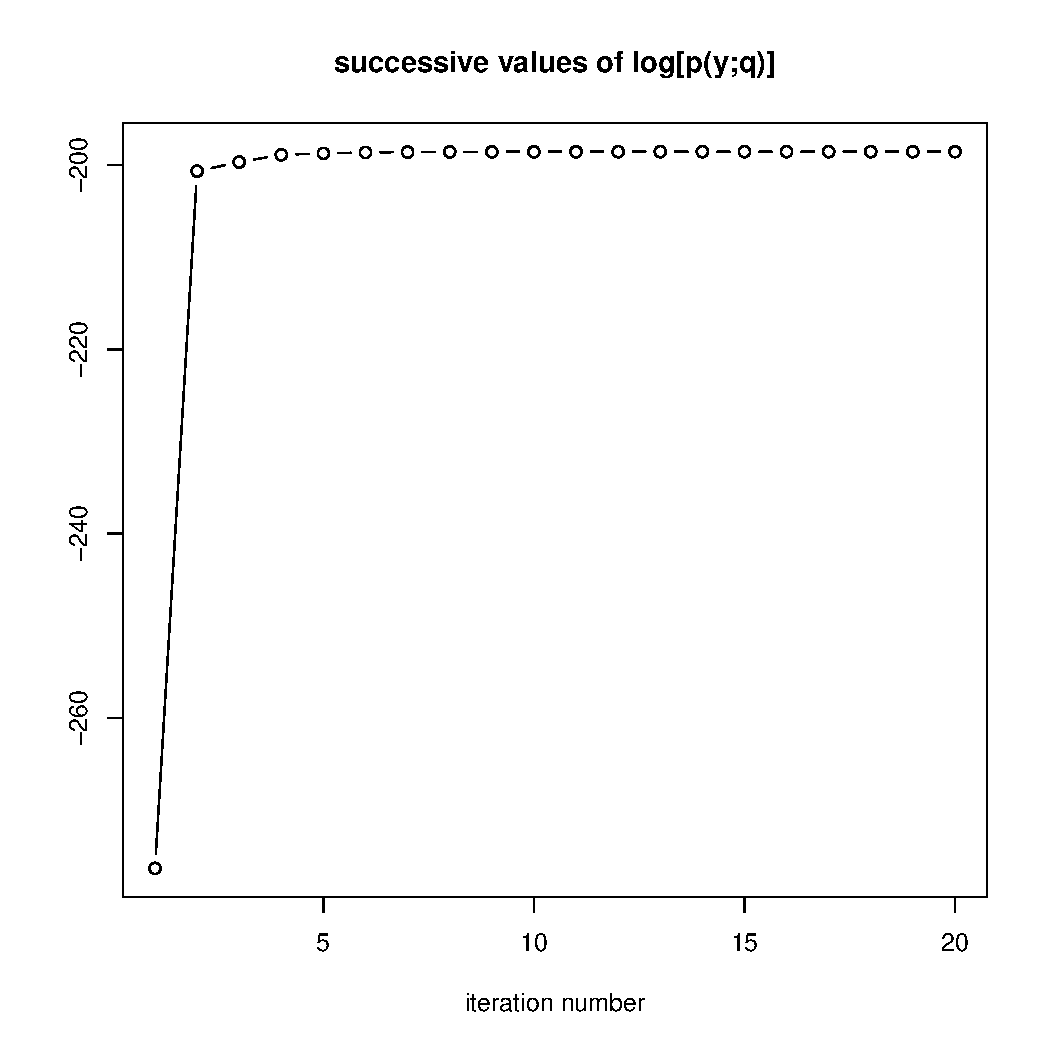
\includegraphics[width=\columnwidth]{logp}}
		\caption{Sample successive variational lower bound for random lag model, when random intercept is the truth. $Y_{ij}\sim N[E(Y_{ij}), \sigma^2]$. \label{f:conv}}
	\end{center}
\end{figure}

The motivating data comes from a study of the effects of exposure to altitude on heart rate and heart rate variability \cite{Meyer2019,MeyerMord2022}. We use the LDLMs and VAICs to select the best covariance structure to describe the relationship between lagged effect of blood oxygen saturation and post-flight heart rate as well as the rate of post-flight supraventricular ectopic heartbeats. For the LDLM with heart rate as the outcome and lagged effect of blood oxygen saturation under both experimental and non-experimental conditions, we find the random lag model to have $VAIC = 404.8$ while the random intercept model has $VAIC = 432.2$. Regardless of decision rule, given that the difference is 27.3, the VAIC suggests that the random lag model induces a better fitting covariance structure for the data when post-flight heart rate is the outcome. For post-flight heart rate variability, we first perform a log-transformation first. Based on this outcome, the random lag model has $VAIC = 120.1$ while the random intercept model has $VAIC = 123.5$. Using the decision rule of selecting the more parsimonious model when the difference in VAICs is less than five, we'd select the random intercept model as the best representation of the covariance structure.


\section{Discussion}

Variational AICs have good discrimination for LDLMs under a number of different decision rules---particularly when the true model is a random lag. The models also exhibit good properties in terms of MISE. Applying the LDLMs and VAIC to the motivating data, we can efficiently select a covariance structure and build inferential models to assess the impact of blood oxygen desaturation, due to altitude exposure, on post-flight heart rate and heart rate variability, measured with rMSSD. 

\bibliographystyle{sdss2020} % Please do not change the bibliography style
\bibliography{fullbib}

\appendix

\section{Variational Bayesian Inference}
\label{a:vbi}
	
	Let $\btheta$ be a vector of parameters and $\by$ denote a vector of observed data. The posterior distribution for $\btheta$ given $\by$ is $p(\btheta | \by) = p(\by, \btheta)\big/p(\by)$. Typically, $p(\by)$ is intractable and posterior estimates need to be obtained algorithmically. For the arbitrary density $q$, $p(\by)$ is bounded below by $\up(\by; \btheta)$ where
	\begin{align*}
		\up(\by; q) = \exp\left[ \int q(\btheta) \log\left\{ \frac{p(\by, \btheta)}{q(\btheta)} \right\} d\btheta \right].
	\end{align*}
	Variational algorithms work by maximizing $\up(\by; q)$ over a class of densities, $q$, that are tractable. This in turn minimizes the Kullback-Leibler Divergence between $q(\btheta)$, and the posterior itself, $p(\btheta | \by)$. Given a partition of $\btheta$ in to $M$ subcomponents, $\{\btheta_1, \ldots, \btheta_M\}$, we use the mean field approximation to construct $q$, specifically $q(\btheta) = \prod_{m = 1}^M q_m(\btheta_m)$. Optimal densities are obtained iteratively with convergence, and therefore minimization, occurring when changes in the variation lower bound, $\up(\by; q)$, become negligible. For a thorough introduction to variational Bayesian techniques with examples, see \cite{OrmerodWand2010}.

\section{Model Derivations and Algorithms}
\label{a:deriv}

The variational lower bounds for the Gaussian model with a random distributed lag is
	\begin{align*}
		\log[ \up(\by; q) ] &= \frac{1}{2}(P + K_0 + K_1 + K_g) - \frac{N}{2}\log(2\pi) \\
			&- \frac{P}{2}\log(\sigma_b^2) + \frac{1}{2}\log\left(|\bSigma_{q(\bbeta, \bgamma^S, \bg^S)}|\right) \\
			&- \frac{1}{2\sigma_b^2}\left[ {\bmu_{q(\bbeta)}}'\bmu_{q(\bbeta)} + \text{tr}\left\{\bSigma_{q(\bbeta)}\right\} \right] \\
			&- a_e\log(b_e) - \left(a_e + \frac{N}{2}\right)\log(B_{q(\sigma^2)}) \\
			&+ \log\left(\Gamma\left(a_e + \frac{N}{2}\right)\right) - \log\left(\Gamma(a_e)\right) \\
			&+ a_0\log(b_0) - \left(a_0 + \frac{K_0}{2}\right)\log(B_{q(\lambda_0)}) \\
			&+ \log\left(\Gamma\left(a_0 + \frac{K_0}{2}\right)\right) - \log(\Gamma(a_0))	\\
			&+ a_1\log(b_1) - \left(a_1 + \frac{K_1}{2}\right)\log(B_{q(\lambda_1)}) \\
			&+ \log\left(\Gamma\left(a_1 + \frac{K_1}{2}\right)\right) - \log(\Gamma(a_1))	\\
			&+ a_g\log(b_g) - \left(a_g + \frac{K_g}{2}\right)\log(B_{q(\lambda_g)}) \\
			&+ \log\left(\Gamma\left(a_g + \frac{K_g}{2}\right)\right) - \log(\Gamma(a_g)).
	\end{align*}
	The lower bound for the random intercept Gaussian model is %similar to the above but with $a_u$, $b_u$, and $K_u$, replacing $a_g$, $b_g$, and $K_g$. Thus the last two lines become $ a_u\log(b_u) - \left(a_u + \frac{K_u}{2}\right)\log(B_{q(\lambda_u)}) + \log\left(\Gamma\left(a_u + \frac{K_u}{2}\right)\right) - \log(\Gamma(a_u))$.
	\begin{align*}
		\log[ \up(\by; q) ] &= \frac{1}{2}(P + K_0 + K_1 + K_u) - \frac{N}{2}\log(2\pi) \\
			&- \frac{P}{2}\log(\sigma_b^2) + \frac{1}{2}\log\left(|\bSigma_{q(\bbeta, \bgamma^S, \bg^S)}|\right) \\
			&- \frac{1}{2\sigma_b^2}\left[ {\bmu_{q(\bbeta)}}'\bmu_{q(\bbeta)} + \text{tr}\left\{\bSigma_{q(\bbeta)}\right\} \right] \\
			&- a_e\log(b_e) - \left(a_e + \frac{N}{2}\right)\log(B_{q(\sigma^2)}) \\
			&+ \log\left(\Gamma\left(a_e + \frac{N}{2}\right)\right) - \log\left(\Gamma(a_e)\right) \\
			&+ a_0\log(b_0) - \left(a_0 + \frac{K_0}{2}\right)\log(B_{q(\lambda_0)}) \\
			&+ \log\left(\Gamma\left(a_0 + \frac{K_0}{2}\right)\right) - \log(\Gamma(a_0))	\\
			&+ a_1\log(b_1) - \left(a_1 + \frac{K_1}{2}\right)\log(B_{q(\lambda_1)}) \\
			&+ \log\left(\Gamma\left(a_1 + \frac{K_1}{2}\right)\right) - \log(\Gamma(a_1))	\\
			&+ a_u\log(b_u) - \left(a_u + \frac{K_u}{2}\right)\log(B_{q(\lambda_u)}) \\
			&+ \log\left(\Gamma\left(a_u + \frac{K_u}{2}\right)\right) - \log(\Gamma(a_u)).
	\end{align*}

Our algorithm is presented in Table~\ref{t:ga} where $C$ is the full design matrix, $C = [X\ L(I_2\otimes\Theta)\ W(I_n \otimes\Theta)]$ for the random distributed lag and $C = [X\ L(I_2\otimes\Theta)\ U]$ for the random intercept. 	
	\begin{table}
		\centering
		\caption{The algorithm for Gaussian outcome with a random distributed lag where $\mathcal{D}  = \text{blockdiag}\left\{ (\sigma_b^2)^{-1} I_{p\times p}, \frac{a_0 + \frac{1}{2} K_0}{B_{q(\sigma_0^2)}} \mathcal{P}, \frac{a_1 + \frac{1}{2} K_1}{B_{q(\sigma_1^2)}} \mathcal{P}, \frac{a_g + \frac{1}{2} K_g}{B_{q(\sigma_g^2)}} \mathcal{P} \right\}$ and $\mathcal{SSY} = \left\{Y - C\bmu_{q(\bbeta, \bgamma^S, \bg^S)} \right\}'\left\{Y - C\bmu_{q(\bbeta, \bgamma^S, \bg^S)} \right\}$. The algorithm for the random intercept model replaces $B_{q(\lambda_g)}$ with $B_{q(\sigma_u^2)}$ and sets $\mathcal{P} = I_{N/2\times N/2}$.\\ \label{t:ga}}
		\begin{tabular}{lll}
			\hline
			\hline
			Initialize: &  & \\
			 & & \\
			$B_{q(\sigma^2)}, B_{q(\sigma_0^2)}, B_{q(\sigma_1^2)}, B_{q(\sigma_g^2)} > 0$ & & \\
			 & & \\
			\hline
			Iterate: &  & \\
			 & & \\
			  $\bSigma_{q(\bbeta, \bgamma^S, \bg^S)} = \left[ \frac{a_e + \frac{N}{2}}{B_{q(\sigma^2)}}C'C + \mathcal{D} \right]^{-1}$ & \\
			 &  & \\
			  $\bmu_{q(\bbeta, \bgamma^S, \bg^S)} = \left( \frac{a_e + \frac{N}{2}}{B_{q(\sigma^2)}}\right)\bSigma_{q(\bbeta, \bgamma^S, \bg^S)}C'Y $ & \\
			 &  & \\
			  $B_{q(\sigma^2)} = b_e + \frac{1}{2}\left[ \mathcal{SSY} + \text{tr}\left\{ C'C \right\}\bSigma_{q(\bbeta, \bgamma^S, \bg^S)} \right]$ & \\
			 &  & \\
			  $B_{q(\lambda_0)} = b_ 0 + \frac{1}{2}\left[ {\bmu_{q(\bgamma_0^S)}}'\bmu_{q(\bgamma_0^S)} + \text{tr}\left\{\frac{a_0 + \frac{1}{2} K_0}{B_{q(\sigma_0^2)}} \mathcal{P} \right\} \right]$ & \\
			 &  & \\
			 $B_{q(\lambda_1)} = b_ 1 + \frac{1}{2}\left[ {\bmu_{q(\bgamma_1^S)}}'\bmu_{q(\bgamma_1^S)} + \text{tr}\left\{\frac{a_1 + \frac{1}{2} K_1}{B_{q(\sigma_1^2)}} \mathcal{P} \right\} \right]$ & \\
			 &  & \\
			  $B_{q(\lambda_g)} = b_ g + \frac{1}{2}\left[ {\bmu_{q(\bgamma_g^S)}}'\bmu_{q(\bgamma_g^S)} + \text{tr}\left\{\frac{a_g + \frac{1}{2} K_g}{B_{q(\sigma_g^2)}}  \mathcal{P} \right\} \right]$ & \\
			 &  & \\
			\multicolumn{2}{l}{until changes in $\log[ \up(\by; q) ]$ are negligible.}  &\\
			 & & \\
			\hline
			\hline
		\end{tabular}
	\end{table}


	
\section{Replication Code}
\label{a:code}
Our replication code can be found in the file \texttt{replication\_code.R} alongside this manuscript.


\end{document}
